\chapter{Project defence}
\label{ch:project_defence}

In what follows a high-level discussion is held on the created code.
Multiple figures and screenshots were made to illustrate the different parts of the project.
Some of these figures are provided in the extra figures list at the end of this report.
For more technical details the reader is invited to read the documentation and comments in the code. 
The \texttt{README.md} file contains a screenshot and discussion of every important part for the end-user.

%------------------------------------

\section{Ideology of CarLovers}
\label{sec:about_carlovers}

CarLovers is a social media platform where registered users can share automobile-related pictures with all other users or a select group of users. 
Other users can interact with the shared post by liking and/or commenting on it.
The ideology and styling (HTML + CSS) of this application are inspired by and sometimes taken from the earlier discussed CarMeets application \citep{github_carmeets} where users can share and plan car meetings.

%------------------------------------

\section{Protecting pages from unwanted users}
\label{sec:protecting_pages}
% Enforcing logged in users only
%% register, login, loginrequired, logoff

As with any project, security is an important aspect.
With web-based applications, the most challenging part is often limiting what request which users can and can't execute.
The general strategy of handling page requests is shown in figure \ref{fig:protecting-pages}.
Due to the use of an MVC pattern, requests sent by the user are processed by a controller.
With Akka Play the controller provides \texttt{Actions} of a certain type to process these requests.
The custom made classes \texttt{AuthenticatedUserAction} and \texttt{AuthenticatedUserActionWithMessageRequest} are responsible for blocking any request that doesn't have a cookie containing a username.
Such actions can thus be used to limit requests to signed-in users, as is done for most of the pages.
The denial page that is shown by these \texttt{Actions} upon a blocked request is the login required page shown in figure \ref{fig:login-requred}.
Sometimes a request is only allowed for a specific user, to process this, the code provided inside the Action should handle the blocking on a per Action basis.

From this login required page, it becomes apparent the user can indeed register an account and log in to his/her account.
Since no database had to be used, the users, and all other objects, are just stored in memory and plain text.
It is noted that this approach may not be used in the real world since such data must be hashed and stored according to various regulations.
Simply having a username cookie is also a very weak account validation mechanism.
The login and register forms are made with Akka Play's form methods and provide various types of validation and error handling.
Figure \ref{fig:login_register} shows the login and register page with some of those validation and error handling features present.
Once the user is logged in, a different menu is shown where the user can log out, add a post or view his/her profile.

\begin{figure}[H]
    \centering
    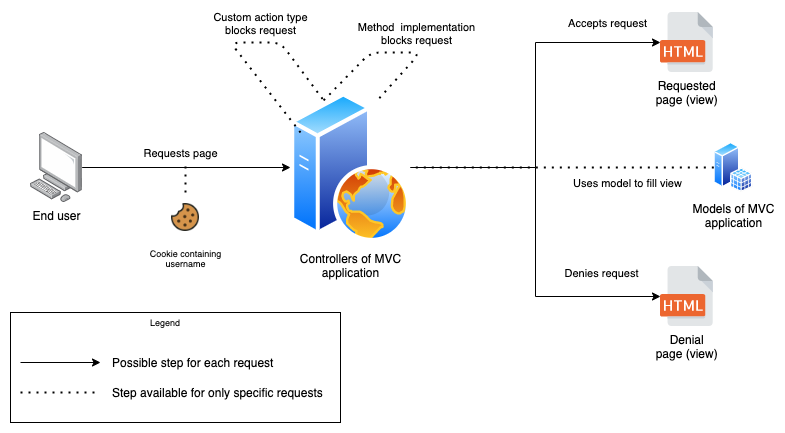
\includegraphics[width=0.8\linewidth]{images/protecting-pages.png}
    \captionsetup{width=0.75\linewidth}
    \captionsetup{justification=centering}
    \caption{Simplified representation of page request procedure. }
    \label{fig:protecting-pages}
\end{figure}


%------------------------------------

\section{Post overview, single post and profile pages}
\label{sec:main_pages}
% Post overview, single post and profile pages
% Reuse of views and sorting

The main pages of the project revolve around viewing posts from users.
Since many of these pages share the same components, these shared components are made available as sub-views.
An obvious such sub-view is \texttt{main}, which provides the header and navigation bar as well as the footer.
As discussed, a different navigation bar (menu), is shown for logged in users.
Less obvious sub-views include the like button (\texttt{postLikeButtonAndCount.scala}), a \textit{post card} which shows a singular post for an overview page (\texttt{postListItem.scala}), comments (\texttt{commentListItem.scala}) and more.
This reuse of sub-views is very visible with the overview and the profile page shown in figure \ref{fig:overview_profile}.
The same sub-view for showing a \textit{post card} can be used but the view is just supplied with a different list of \texttt{PostWithInfo} objects, e.g. from a specific user or ordered differently.
Such a \texttt{PostWithInfo} object contains a \texttt{Post} and \texttt{Visibility} object as well as a list of \texttt{Likes} and \texttt{Comments}.
The MVC pattern is present: after a user request, the controller sets up the model so that the view can display information to the end-user.
The controller is thus responsible for reasoning about which \texttt{PostWithInfo} objects should be visible to the user, based on the information from the \texttt{Visibility} object.
Figure \ref{fig:homedifferent} shows that the homepage for two users can be different based on the \texttt{Visibility} information.

Figure \ref{fig:overview} shows that a user can like a post from the overview page and sees at most three comments per post on the overview page.
If the post in question is placed by the logged-in user, the delete and edit buttons are also present.
The user is forwarded to the single page of a post when clicking read more, the image, or the like button.
As shown in figure \ref{fig:single}, all comments can be read on this single post page and a comment can be placed by the user.

%------------------------------------
\clearpage
\section{Managing and visibility of posts}
\label{sec:managing}

The last important part of the puzzle for this project is managing posts.
Compared to previous forms where Akka Play neatly created instances of objects upon form bind, uploading a file and working with lists provides some manual work.
Luckily the Akka Play documentation pointed in the right direction\footnote{\url{https://www.playframework.com/documentation/2.8.x/ScalaFileUpload}}.
The add post form is shown in figure \ref{fig:addpost} and a correct \texttt{PostWithInfo} object is made in two different parts.
Firstly the standard form approach is used to create a \texttt{Post} object and validate the description field by using hidden fields in a pre-filled form for the system-generated values.
For the image and visibility settings, the form body is manually checked for correctness and error messages are shown manually through view settings.
The code in the \texttt{PostController} is well documented and explains this procedure in greater detail.

After submitting the form successfully, the user is forwarded to the just created post.
The edit visibility page is shown in figure \ref{fig:editpost} and demonstrates that also this form is pre-filled with the settings chosen on post creation.
Deleting the post simply takes the user to his profile page after a successful deletion with a flash message notifying him of the successful deletion.





%------------------------------------
\section{Other caveats}
\label{sec:caveats}

This assignment has proven to be rather lengthy and explaining each portion in great detail is simply not possible in a document that is already over the page limit.
The \texttt{README} file provides screenshots for each important step and discusses briefly what is important in each step.
As always, the code is very well documented and the reader is invited to take a look at specific methods to have a better understanding of how certain parts of the code work.